\documentclass[../main.tex]{subfiles}
\begin{document}
\chapter{Integration}
\section{Basics}
\subsection{Defining the Integral}
We want to define $\int_{a}^{b} f(x) \d{x}$ as the signed area enclosed by $f$ between $a$ and $b$.
This is easy if the region enclosed by the graph is a nice geometric shape, if not, we can try approximating the area using rectangles.
Two ways we could do this are using the left and right Riemann sums:
\begin{center}
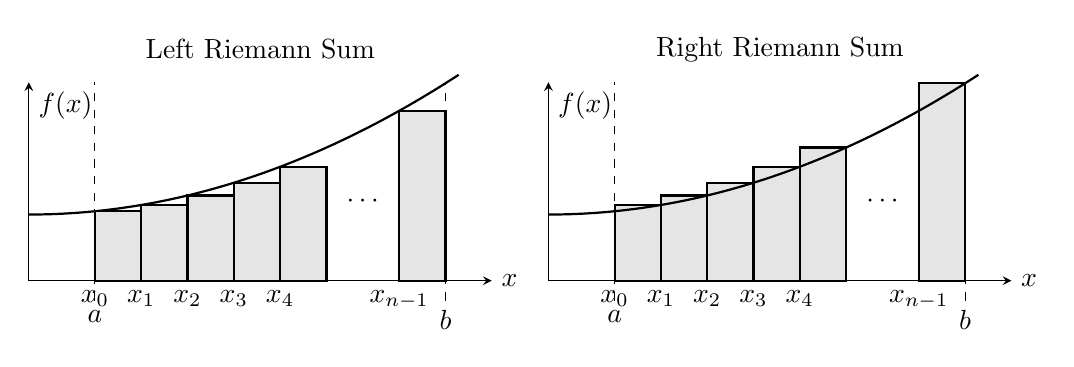
\begin{tikzpicture}[scale=1.2, >=stealth]
  \begin{scope}[scale=0.7]
    \node at (3.5, 3.5) {Left Riemann Sum};
    \draw[->] (0,0) -- (7,0) node[right] {$x$};
    \draw[->] (0,0) -- (0,3) node[below right] {$f(x)$};

    \draw[thick, domain=0:6.5, smooth, variable=\x] plot ({\x}, {0.05*\x^2 + 1});

    \node[below] at (1,-0.3) {$a$};
    \draw[dashed] (1,-0.3) -- (1,3);
    \node[below] at (6.3,-0.3) {$b$};
    \draw[dashed] (6.3,-0.3) -- (6.3,3);

    \def\dx{0.7}
    \foreach \i in {0,1,2,3,4} {
      \pgfmathsetmacro{\xleft}{1 + \i*\dx}
      \pgfmathsetmacro{\height}{0.05*\xleft^2 + 1}
      \fill[gray!20] (\xleft,0) rectangle ({\xleft+\dx}, {\height});
      \draw[thick] (\xleft,0) rectangle ({\xleft+\dx}, {\height});
      \node[below] at (\xleft,0) {$x_\i$};
    }

    \node at (5.05,1.2) {$\cdots$};

    \pgfmathsetmacro{\xfinal}{5.6}
    \pgfmathsetmacro{\hfinal}{0.05*\xfinal^2 + 1}
    \node[below] at (\xfinal,0) {$x_{n-1}$};
    \fill[gray!20] (\xfinal,0) rectangle ({\xfinal+\dx}, {\hfinal});
    \draw[thick] (\xfinal,0) rectangle ({\xfinal+\dx}, {\hfinal});
  \end{scope}

  \begin{scope}[xshift=5.5cm, scale=0.7]
    \node at (3.5, 3.5) {Right Riemann Sum};
    \draw[->] (0,0) -- (7,0) node[right] {$x$};
    \draw[->] (0,0) -- (0,3) node[below right] {$f(x)$};


    \node[below] at (1,-0.3) {$a$};
    \draw[dashed] (1,-0.3) -- (1,3);
    \node[below] at (6.3,-0.3) {$b$};
    \draw[dashed] (6.3,-0.3) -- (6.3,3);

    \def\dx{0.7}
    \foreach \i in {0,1,2,3,4} {
      \pgfmathsetmacro{\xleft}{1 + \i*\dx}
      \pgfmathsetmacro{\height}{0.05*(\xleft + \dx)^2 + 1}
      \fill[gray!20] (\xleft,0) rectangle ({\xleft+\dx}, {\height});
      \draw[thick] (\xleft,0) rectangle ({\xleft+\dx}, {\height});
      \node[below] at (\xleft,0) {$x_\i$};
    }

    \node at (5.05,1.2) {$\cdots$};

    \pgfmathsetmacro{\xfinal}{5.6}
    \pgfmathsetmacro{\hfinal}{0.05*(\xfinal + \dx)^2 + 1}
    \node[below] at (\xfinal,0) {$x_{n-1}$};
    \fill[gray!20] (\xfinal,0) rectangle ({\xfinal+\dx}, {\hfinal});
    \draw[thick] (\xfinal,0) rectangle ({\xfinal+\dx}, {\hfinal});

    \draw[thick, domain=0:6.5, smooth, variable=\x] plot ({\x}, {0.05*\x^2 + 1});
  \end{scope}
\end{tikzpicture}
\end{center}
We first need to define how we can split up the real line between the \textit{integration bounds $a$ and $b$}:
\begin{definition}[Partition/Dissection]
  A \textit{partition} $\mathcal{P}$ or \textit{dissection} of an interval $[a, b]$ is a \textbf{finite subset} of $[a, b]$ with the requirement that $a, b \in \mathcal{P}$.

  We often write $\mathcal{P} = \{x_0, \ldots, x_n\}$ where $a = x_0 < x_1 < \cdots < x_n = b$ and $x_i \in [a, b]\ \forall i$.
\end{definition}
Instead of the left and right Riemann sums, we will instead use the \textit{upper and lower} Riemann sums.
These use the supremum/infimum respectively of $f$ over each interval between the points of a partition.
\begin{definition}[Upper/Lower Riemman Sums]
  For a bounded $f: [a, b] \to \R$ and partition $\mathcal{P}$ of $[a, b]$, we define the \textit{Lower Riemann sum} as:
  \[
    L(f, \mathcal{P}) = \sum_{j = 1}^{n} (x_j - x_{j - 1}) \inf_{x \in I_j} f(x)
  \]
  and the \textit{Upper Riemann sum} as:
  \[
    U(f, \mathcal{P}) = \sum_{j = 1}^{\infty} (x_j - x_{j - 1}) \sup_{x \in I_j} f(x)
  \]
  where $I_j = [x_{j - 1}, x_{j}]$.
\end{definition}
\begin{example}
  Consider again the \textit{Dirichlet function} from \cref{dirichletFunction}:
  \label{dirichletUpperLower}
  \[
    f(x) = 1_\Q(x) = \begin{cases}
    1 & \text{ if } x \in \Q \\
    0 & \text{ if } x \notin \Q
    \end{cases}
  \]
  No matter what $\mathcal{P}$ is, since $\Q$ is dense in $\R$, $I_j = [x_{j - 1}, x_j]$ will always contain a rational and an irrational number, hence:
  \[
    \sup_{x \in I_j} f(x) = 1 \text{ and } \inf_{x \in I_j} f(x) = 1
  \]
  and so:
  \begin{align*}
    U(f, \mathcal{P}) &= 1 \cdot \sum_{j = 1}^{n} (x_j - x_{j - 1}) \\
                       &= x_1 - x_0 + x_2 - x_1 + \cdots + x_n - x_{n - 1} \\
                       &= x_n - x_0 = b - a = 1 - 0 = 1 \\
    L(f, \mathcal{P}) &= 0 \cdot \sum_{j = 1}^{n} (x_j - x_{j - 1}) = 0 \\
  \end{align*}
\end{example}
For bounded $f$, $\exists k \text{ s.t. } \sup_{x \in [a, b]} |f(x)| = k$.
Since $\sup_{x \in I_j} f(x) \leq \sup_{x \in [a, b]} f(x)$, we can bound $U(f, \mathcal{P})$ as:
\begin{align*}
  U(f, \mathcal{P}) &\leq \sum_{j = 1}^{n} (x_{j} - x_{j - 1}) \sup_{x \in [a, b]} |f(x)|  \\
                     &\leq K \sum_{j = 1}^{n} (x_j - x_{j - 1}) = k(b - a)
\end{align*}
and since $\inf_{x \in I_j} f(x) \geq \inf_{x \in [a, b]} f(x) \geq -\sup_{x \in [a, b]} |f(x)| = -k$
\begin{align*}
  L(f, \mathcal{P}) &\geq \sum_{j = 1}^{n} (x_{j} - x_{j -1}) \left[- \sup_{x \in [a, b]} |f(x)|\right] \\
                     &= -k(b - a)
\end{align*}
From the definition, we clearly have that $U(f, \mathcal{P}) \geq L(f, \mathcal{P})$ and so:
\[
  -k(b - a) \leq L(f, \mathcal{P}) \leq U(f, \mathcal{P}) \leq k(b - a)
\]
Geometrically, this is saying that $L$ and $U$ are bounded below by a rectangle from $a$ to $b$ of height $-k$ and above by a rectangle from $a$ to $b$ of height $k$ where $k = \sup_{x \in [a, b]} f(x)$.

Therefore, the sets:
\[
  \{L(f, \mathcal{P}): \mathcal{P} \text{ is a partition of $[a, b]$}\} \text{ and } \{U(f, \mathcal{P}): \mathcal{P} \text{ is a partition of $[a, b]$}\}
\]
are both bounded.
They are also non empty since as $\{a,b\}$ is always a partition of $[a, b]$.
This means that they both have supremum and infimum.
\begin{definition}[Upper/Lower Integral]
  Let $f: [a, b] \to \R$ be a bounded function.
  We define the \textit{lower Riemann integral} of $f$ in $[a, b]$ as:
  \[
    I_{*}(f) = \sup_{\mathcal{P}} L(f, \mathcal{P})
  \]
  and the \textit{upper Riemann integral} of $f$ in $[a, b]$ as:
  \[
    I^{*}(f) = \inf_{\mathcal{P}} U(f, \mathcal{P})
  \]
\end{definition}
\begin{definition}[Riemman Integrable]
  We say that bounded function $f: [a, b] \to \R$ is \textit{Riemann integrable} if $I_{*}(f) = I^{*}(f)$ and then define:
  \label{integralDef}
  \[
    I(f) = \int_{a}^{b} f(x) \d{x} = I_{*}(f) = I^{*}(f)
  \]
  to be the \textit{Riemann integral of $f$ from $a$ to $b$}.
\end{definition}
\begin{remark}[Intuition]
  This is like saying the largest of the pessimistic approximations agrees with the smallest of the optimistic approximations.
\end{remark}
\begin{remark}
  By convention, if we change the order of the bounds, then the sign of the integral flips, that is:
  \[
    \int_{a}^{b} f(x) \d{x} = - \int_{b}^{a} f(x) \d{x}
  \]
\end{remark}
\begin{example}
  Consider again the Dirichlet indicator function from \cref{dirichletUpperLower}.
  Its upper and lower integrals are $I^{*}(f) = 1$ and $I_{*}(f) = 0$, so $f$ is not integrable.
\end{example}
\subsection{Properties of Partitions}
Intuition suggests that a finer partition leads to a better estimate for the area, this turns out to be true:
\begin{lemma}
  If $\mathcal{P}$ and $\mathcal{P}'$ be partitions of $[a, b]$ such that $\mathcal{P} \subseteq \mathcal{P}'$, that is, $\mathcal{P}'$ is a \textit{refinement of $\mathcal{P}$}, then:
  \label{refinementInequality}
  \[
    L(f, \mathcal{P}) \leq L(f, \mathcal{P'}) \leq U(f, \mathcal{P}') \leq U(f, \mathcal{P})
  \]
  for every bounded $f: [a, b] \to \R$.
\end{lemma}
\begin{proof}
  For now, assume that $\mathcal{P}$ and $\mathcal{P}'$ differ by one point only.
  Take $\mathcal{P} = \{x_0, \ldots, x_n\}$.
  Since $\mathcal{P}'$ differs by one point, $\mathcal{P}' = \mathcal{P} \cup \{y\}$ where $y \in (x_{k - 1}, x_k)$ for some $k \in \{1, \ldots, n\}$.
  In this case, we then have:
  \[
    \sup_{x \in [x_{k - 1}, y]} f(x),\ \sup_{x \in [y, x_k]} f(x) \leq \sup_{x \in [x_{k - 1}, x_k]} f(x)
  \]
  and so:
  \begin{align*}
    (y - x_{k - 1})\sup_{x \in [x_{k - 1}, y]} f(x) + (x_k - y) \sup_{x \in [y, x_k]} f(x) &\leq (y - x_{k - 1}+ x_k - y) \sup_{x \in [x_{k - 1}, x_k]} f(x) \\
                                                                                           &= (x_k - x_{k - 1}) \sup_{x \in [x_{k - 1}, x_k]}  f(x)
  \end{align*}
  The sum for $U(f, \mathcal{P}')$ has the terms on the left hand side of the inequality, whereas the sum for $U(f, \mathcal{P})$ instead has the term on the right hand side of the inequality, otherwise, the sums are the same as $\mathcal{P}$ and $\mathcal{P}'$ differ only by one point.
  Therefore, $U(f, \mathcal{P}') \leq U(f, \mathcal{P})$.

  Similarly, using the infimum in the first line instead yields:
  \[
    \inf_{x \in [x_{k - 1}, y]} f(x),\ \inf_{x \in [y, x_k]} f(x) \geq \inf_{x \in [x_{k - 1}, x_k]} f(x)
  \]
  So using a similar argument, we get that $L(f, \mathcal{P}') \geq L(f, \mathcal{P})$.
  Therefore, if $\mathcal{P}'$ and $\mathcal{P}$ differ by one point, the result holds since the middle inequality was shown previously.

  Since partitions are finite subsets, $\mathcal{P}'$ and $\mathcal{P}$ can differ only by a finite number of points.
  So if $\mathcal{P}' \setminus \mathcal{P} = \{y_1, \ldots, y_n\}$, then we can just repeat this argument $n$ times to yield the result.
\end{proof}
\begin{corollary}
  If $\mathcal{P}_1$ and $\mathcal{P}_2$ are partitions of $[a, b]$, then:
  \label{partitionRelation}
  \[
    L(f, \mathcal{P}_1) \leq U(f, \mathcal{P}_2)
  \]
  for every bounded $f: [a, b] \to \R$.
\end{corollary}
\begin{remark}[Note]
  Neither of $\mathcal{P}_1$ and $\mathcal{P}_2$ have to be a refinement of the other for this to hold.
\end{remark}
\begin{proof}
  Since $\mathcal{P}_1, \mathcal{P}_2 \subseteq \mathcal{P}_1 \cup \mathcal{P}_2$, $\mathcal{P}_1$ and $\mathcal{P}_2$ are both refinements of $\mathcal{P}_1 \cup \mathcal{P}_2$.
  Applying \cref{refinementInequality} twice, we have:
  \[
    L(f, \mathcal{P}_1) \leq U(f, \mathcal{P}_1 \cup \mathcal{P}_2) \leq U(f, \mathcal{P}_2)
  \]
  which is the desired result.
\end{proof}
\begin{corollary}
  If $f: [a, b] \to \R$ is bounded, then $I_*(f) \leq I^{*}(f)$.
  \label{upperLowerIntegralRelation}
\end{corollary}
\begin{proof}
  By \cref{partitionRelation}, if we fix some partition $\mathcal{P}$, then $L(f, \mathcal{P}) \leq U(f, \mathcal{P}')$ for all partitions $\mathcal{P}'$.
  Therefore:
  \[
    L(f, \mathcal{P}) \leq \inf_{\mathcal{P}'} U(f, \mathcal{P}')
  \]
  Since $\mathcal{P}$ was arbitrary, this relation is true for all partitions $\mathcal{P}$ and so
  \begin{align*}
    \sup_{\mathcal{P}} L(f, \mathcal{P}) &\leq \inf_{\mathcal{P}'} U(f, \mathcal{P'}) \\
    \implies I_{*}(f) &\leq I^{*}(f)
  \end{align*}
\end{proof}
\begin{remark}
  This means that $f$ is integrable if and only if $I_{*}(f) \geq I^{*}(f)$ since we always have $I_{*}(f) \leq I^{*}(f)$ for bounded $f$.
\end{remark}
\subsection{Integrability of General Functions}
Is there another definition for Riemann integrability that is more akin of the others we have seen so far in the course such as those for continuity and limits?

We would like to show that for any threshold, we can always find a partition of $[a, b]$ so that the difference between the upper and lower Riemann sums is below the threshold.
\begin{proposition}[Riemman Integrability Critereon]
  Let $f: [a, b] \to \R$ be bounded.

  $f$ is Riemann integrable if and only if:
  \label{integrabilityCritereon}
  \[
    \forall \varepsilon > 0\ \exists \mathcal{P} = \mathcal{P}(\varepsilon) \text{ a partition of } [a, b] \text{ s.t. } U(f, \mathcal{P}) - L(f, \mathcal{P}) < \varepsilon
  \]
\end{proposition}
\begin{proof}
  \begin{proofdirection}{Assume $f$ is Riemann integrable}
    From the definition of supremum and infimum, for any $\varepsilon > 0$, we can always find $\mathcal{P}$ and $\mathcal{P}'$ such that:
    \[
      U(f, \mathcal{P}) \leq I^{*}(f) + \frac{\varepsilon}{2} \text{ and } L(f, \mathcal{P}') \geq I_{*}(f) - \frac{\varepsilon}{2}
    \]
    Taking the difference:
    \[
      U(f, \mathcal{P}) - L(f, \mathcal{P'}) \leq \varepsilon
    \]
    To conclude, we need to find a single partition where this difference is smaller than $\varepsilon$.
    Let $\mathcal{P}'' = \mathcal{P} \cup \mathcal{P}'$.
    We see that $\mathcal{P} \subseteq \mathcal{P}$ so $\mathcal{P}''$ is a refinement of $\mathcal{P}$, therefore, by \cref{refinementInequality}, $U(f, \mathcal{P}'') \leq U(f, \mathcal{P})$.
    Similarly, $\mathcal{P}''$ is a refinement of $\mathcal{P}'$ and so $L(f, \mathcal{P}'') \geq L(f, \mathcal{P}')$.

    Combining these inequalities, we have:
    \[
      U(f, \mathcal{P}'') - L(f, \mathcal{P}'') \leq U(f, \mathcal{P}) - L(f, \mathcal{P}') \leq \varepsilon
    \]
  \end{proofdirection}
  \begin{proofdirection}{Assume that we can always find such a partition}
    So for any $\varepsilon > 0$, $\exists \mathcal{P}$ such that $U(f, \mathcal{P}) - L(f, \mathcal{P}) < \varepsilon$.
    We also know that for any partition $\mathcal{P}$, $U(f, \mathcal{P}) \geq I^{*}(f)$ and $L(f, \mathcal{P}) \leq I_*(f)$.

    Therefore:
    \[
      0 \leq I^{*}(f) - I_{*}(f) \leq U(f, \mathcal{P}) - L(f, \mathcal{P}) < \varepsilon
    \]
    Hence:
    \[
      0 \leq I^{*}(f) - I_{*}(f) < \varepsilon
    \]
    Since $\varepsilon$ can be arbitrarily small, $I^{*}(f) = I_{*}(f)$ and so $f$ is Riemann integrable.
  \end{proofdirection}
\end{proof}
\begin{proposition}
  Let $f: [a, b] \to \R$ be bounded.
  $f$ is Riemann integrable if and only if there exists a sequence of partitions $(\mathcal{P}_n)$ of $[a, b]$ such that:
  \label{integrableSequence}
  \[
    U(f, \mathcal{P}_n) - L(f, \mathcal{P}_n) \to 0 \text{ as } n \to \infty
  \]
\end{proposition}
\begin{proof}
  \begin{proofdirection}{Assume $f$ is Riemann integrable}
    Let $\varepsilon = \frac{1}{n}$ for some fixed $n \in \N$, by \cref{integrabilityCritereon}, $\exists \mathcal{P}_n$ such that $U(f, \mathcal{P}_n) - L(f, \mathcal{P}_n) < \frac{1}{n}$.
    We can use this to construct a sequence of events $(\mathcal{P}_n)$ by carrying out the above process for every $n \in \N$.
    By construction $0 \leq U(f, \mathcal{P}_n) - L(f, \mathcal{P}_n) \leq \frac{1}{n}$, so taking $n \to \infty$, we see that $U(f, \mathcal{P}_n) - L(f, \mathcal{P}_n) \to 0$.
  \end{proofdirection}
  \begin{proofdirection}{Assume there exists such a sequence of partitions}
    Let $a_n = U(f, \mathcal{P}_n) - L(f, \mathcal{P}_n) \geq 0$.
    Since $a_n \to 0$, for any $\varepsilon > 0\ \exists N(\varepsilon)$ such that:
    \[
      U(f, \mathcal{P}_n) - L(f, \mathcal{P}_n) = |a_n| < \varepsilon\ \forall n \geq N
    \]
    So defining $\mathcal{P}'(\varepsilon) = \mathcal{P}_{N(\varepsilon)}$:
    \[
      \forall \varepsilon > 0\ \exists \mathcal{P}'(\varepsilon) \text{ s.t. } U(f, \mathcal{P}') - L(f, \mathcal{P}') < \varepsilon
    \]
    and so $f$ is integrable by \cref{integrabilityCritereon}.
  \end{proofdirection}
\end{proof}
\begin{example}[Examples of Integrable Functions]
  \begin{enumerate}
    \item Let $f: [0, 1] \to \R,\ x \mapsto x$ and define $\mathcal{P}_n = \{0, \frac{1}{n}, \ldots, \frac{n - 1}{n}, 1\}$.

      By definition:
      \begin{align*}
        U(f, \mathcal{P}_n) &= \sum_{j = 1}^{n} \left(\frac{j}{n} - \frac{j - 1}{n}\right) \sup_{x \in [\frac{j - 1}{n}, \frac{j}{n}]} x \\
                            &= \frac{1}{n} \sum_{j = 1}^{n} \frac{j}{n} \\
                            &= \frac{1}{n^2} \cdot \frac{1}{2}n(n + 1) = \frac{1}{2}\left(1 + \frac{1}{n}\right)
      \end{align*}
      Similarly:
      \begin{align*}
        L(f, \mathcal{P}_n) &= \frac{1}{n} \sum_{j = 1}^{n} \inf_{[\frac{j - 1}{n}, \frac{j}{n}]} x \\
                            &= \frac{1}{n} \sum_{j = 1}^{n} \frac{(j - 1)}{n} \\
                            &= \frac{1}{n^2} \cdot \frac{1}{2}n(n - 1) = \frac{1}{2}\left(1 - \frac{1}{n}\right)
      \end{align*}

      \textbf{Using Original Definition -- \Cref{integralDef}}\par
      Since the set of $\{\mathcal{P}_n: n \in \N\}$ is a subset of the set of all possible partitions, we have:
      \[
        I_{*}(f) = \sup_{\mathcal{P}} L(f, \mathcal{P}) \geq \sup_{n \in \N} L(f, \mathcal{P}_n) = \frac{1}{2}
      \]
      and:
      \[
        I^{*}(f) = \inf_{\mathcal{P}} U(f, \mathcal{P}) \leq \inf_{n \in \N} U(f, \mathcal{P}_n) = \frac{1}{2}
      \]
      Thus $I^{*}(f) \leq I_{*}(f)$, so by \cref{upperLowerIntegralRelation}, $I_{*}(f) = I^{*}(f)$.
      So $f$ is integrable and $\int_{0}^{1} f(x) \d{x} = \frac{1}{2}$.

      \textbf{Using Riemann Integrability Sequence Criterion -- \cref{integrableSequence}}\par
      Using $(\mathcal{P}_n)$ as our sequence of events, we see that:
      \[
        U(f, \mathcal{P}_n) - L(f, \mathcal{P}_n) = \frac{1}{n} \to 0 \text{ as $n \to \infty$}
      \]
      So $f$ is integrable.
    \item Define:
      \[
        f: [0, 1] \to \R,\ x\mapsto \begin{cases}
        0 & \text{ if } x\leq \frac{1}{2} \\
        1 & \text{ if } x > \frac{1}{2}
        \end{cases}
      \]
      Taking $\mathcal{P}_n$ as before for $n \geq 3$, for $k \in \{1, \ldots, n\}$ we have:
      \[
        \sup_{x \in [x_{k - 1}, x_{k}]} f(x) - \inf_{x \in [x_{k - 1}, x_{k}]} f(x) = \begin{cases}
        1 & \text{ if } \frac{1}{2} \in [x_{k - 1}, x_{k}] \\
        0 & \text{otherwise}
        \end{cases}
      \]
      Since $\frac{1}{2}$ can be in exactly one interval of the partition:
      \begin{align*}
        U(f, \mathcal{P}_n) - L(f, \mathcal{P}_n) &= \sum_{j = 1}^{n} (x_j - x_{j - 1}) \left[\sup_{x \in I_j} f(x) - \inf_{x \in I_j} f(x)\right] \\
                                                  &= \sum_{j = 1}^{n} \frac{1}{n} \left[\sup_{x \in I_j} f(x) - \inf_{x \in I_j} f(x)\right] \\
                                                  &= \frac{1}{n} \cdot 1 \to 0 \text{ as } n \to \infty
      \end{align*}
      So by \cref{integrableSequence}, $f$ is integrable.
  \end{enumerate}
\end{example}
It is quite tedious to check if a function is integrable using these methods so it would be useful to know what classes of functions are integrable.
\begin{proposition}[Monotone $\implies$ Integrable]
  If $f: [a, b] \to \R$ is monotone, then $f$ is integrable.
\end{proposition}
\begin{proof}
  Since $f$ is monotone, $f$ is bounded by $\max\{f(a), f(b)\}$.
  By definition:
  \[
    U(f, \mathcal{P}) -L(f, \mathcal{P}) = \sum_{j = 1}^{n} \left[\sup_{x \in I_{j}} f(x) - \inf_{x \in I_j} f(x)\right]|I_j|
  \]
  Continued next lecture.
\end{proof}
\end{document}
